\documentclass{article}
\usepackage[utf8]{inputenc}
\usepackage{graphicx}
\title{Beam Geometries and their Strength}
\author{Matthew Zhang}
\date{June 2018}

\begin{document}

\maketitle


\section*{Abstract}
This experiment was conducted in order to answer a question concerning torques and forces: How do well do different shapes of beams resist bending due to a load being placed on their end? In class the concept of torques had already been introduced as a type of "rotational force". The experiment tested 3D-printed beams of various different profiles by hanging weights off of their ends when supported cantilever on one end. This experiment subjected various objects to a constant torque and examined how they performed mechanically due to the torque. The experiment found that profiles containing more material tended to perform better, with an increased effectiveness if the material is located in the dimension of the load.



\section*{Procedure}
\begin{enumerate}
\item 
Take a beam and clamp it to the table, making sure that the end hangs off 85 mm off of the edge of the table. Orient it so that the hole in the beam goes sideways, and is also hanging off the table
\item
Tie a string around the hole in the beam and attach two 200g weights to the end of the string
\item
Place a meter stick next to the bending beam to use as a horizontal reference, and measure the amount of bending by using the caliper to measure dimension along the vertical axis from the top of the meterstick to the bottom of the end of the beam
Record this value
\item
Use a scale to measure the mass of the beam
\item
Repeat steps 1-4 for every single beam
\item
Measure and record the height of the meterstick
\end{enumerate}
\begin{center}
	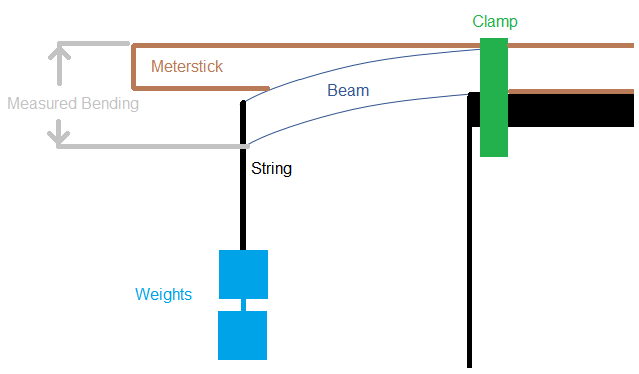
\includegraphics[width=.8\linewidth]{whysicDiagram.png}
\end{center}

\section*{Data}


\section*{Conclusion}

\end{document}
